%%
%% 章:TikZ
%%------------------------------------------------------------------------------------------------------------------------------%%
\chapter{Ti\textit{k}Z}
Ti\textit{k}Z\footnote{Ti\textit{k}Z の読み方は特に決まっていないが「ティックジィー」「ティックス」などと読まれている。} は\TeX{}の中で使える強力な\ruby{描画}{ドロー}コマンド群である。
従来の picture 環境、\MP、Asymptote、PSTricks に置き換えて使うことができる。
統計ツール R やグラフ作成ツール gnuplot と組み合わせれば、より高度なグラフを描くことができる。
%%
%% 節:PGF/TikZ とは?
%%--------------------------------------------------------------------------------------------------------------------%%
\section{PGF/Ti\textit{k}Z とは?}
Ti\textit{k}Z は\TeX{}の中で使える強力な\ruby{描画}{ドロー}コマンド群である。
作者は、スライド作成用パッケージ Beamer の作者としても有名な Till Tantau 氏である。\\

Ti\textit{k}Z は見ての通り \textit{k} だけイタリック体で記述する。
名前の由来は Ti\textit{k}Z ist \textit{kein} Zeichenprogramm(Ti\textit{k}Z はドローツールでは\.な\.い)である(再帰的な略語)。
従来の\LaTeX{}の picture 環境を強力にしたもので、機能的には \MP、Asymptote、PSTrick に近いのだが、バックエンドとして PGF(Portable Graphics Format)という仕組みを使っており、PostScript を介さないのでトラブルが起きにくく、日本語の問題も生じない。
また、独立なプログラムを使わず\TeX{}の中に直接記述できるのも大きな利点である。
Beamer でも PGF を使っている。\\

Ti\textit{k}Z を使うには、$\epsilon$-\TeX{}拡張された\TeX{}が必要となるが、最近のものであれば大丈夫である。
PGF/Ti\textit{k}Z の詳しい PDF マニュアルは、\TeX{} Live を入れたシステムなら、ターミナルに texdoc tikz と打ち込めば表示される。
%%
%% 節:TikZ の基本
%%--------------------------------------------------------------------------------------------------------------------%%
\section{Ti\textit{k}Z の基本}
Ti\textit{k}Z を使うには、次の例のように、プリアンブルに \verb'\usepackage{tikz}' と記述する。
更に、dvipdfmx で PDF 化する場合(通常の日本語文書処理の場合)は、ドキュメントクラスのオプションに dvipdfmx と記述する\footnote{あるいは、dvipdfmx オプションを付加した graphicx と xcolor を先に読み込んでおく。}。\\

簡単な例を試してみる。
\vspc{+0.50zw}\begin{mdframed}[roundcorner=0.50zw,leftmargin=3.00zw,rightmargin=3.00zw,skipabove=0.40zw,skipbelow=0.40zw,innertopmargin=4.00pt,innerbottommargin=4.00pt,innerleftmargin=5.00pt,innerrightmargin=5.00pt,linecolor=gray!020,linewidth=0.50pt,backgroundcolor=gray!20]
\begin{verbatim}
\documentclass[dvipdfmx]{jsarticle}
\usepackage{tikz}
\begin{document}
\tikz\draw(0,0)--(0.1,0.2)--(0.2,0.0)--(0.3,0.2)--(0.4,0.0);
\end{document}
\end{verbatim}
\end{mdframed}\vspc{-0.70zw}
これで「\tikz\draw(0,0)-- (0.1, 0.2)-- (0.2,0.0)-- (0.3,0.2)-- (0.4,0.0);」のような出力が得られる。
\verb'(0,0)' などは座標であり、デフォルトの単位は \ajLig{cm} だが \verb'(12mm,3pt)' のように\TeX{}が理解する単位を付けることもできる。
p\TeX{}専用の zw などの単位は使えないが、本文フォントの 1zw に相当する長さ \verb'\Cwd' が日本語ドキュメントクラスの中で定義されているので、例えば 3zw なら \verb'3\Cwd' と書くことができる。\\

このように \verb'\draw' は点を結んで折れ線を描く。\enlargethispage{+0.85zw}
\verb'draw' 文の最後にはセミコロンが必要となる。
複数の \verb'\draw' が存在する場合は、
\vspc{+0.50zw}\begin{mdframed}[roundcorner=0.50zw,leftmargin=3.00zw,rightmargin=3.00zw,skipabove=0.40zw,skipbelow=0.40zw,innertopmargin=4.00pt,innerbottommargin=4.00pt,innerleftmargin=5.00pt,innerrightmargin=5.00pt,linecolor=gray!020,linewidth=0.50pt,backgroundcolor=gray!20]
\begin{verbatim}
\tikz{\draw(0,0)-- (10pt,10pt); \draw(0,10pt)-- (10pt,0);}
\end{verbatim}
\end{mdframed}\vspc{-0.70zw}
のように中括弧で囲むか、あるいは、
\vspc{+0.50zw}\begin{mdframed}[roundcorner=0.50zw,leftmargin=3.00zw,rightmargin=3.00zw,skipabove=0.40zw,skipbelow=0.40zw,innertopmargin=4.00pt,innerbottommargin=4.00pt,innerleftmargin=5.00pt,innerrightmargin=5.00pt,linecolor=gray!020,linewidth=0.50pt,backgroundcolor=gray!20]
\begin{verbatim}

\begin{tikzpicture}
  \draw(0,0) -- (10pt,10pt);
  \draw(0,10pt) -- (10pt,0);
\end{tikzpicture}
\end{verbatim}
\end{mdframed}\vspc{-0.70zw}
のように tikzpicture 環境を用いる。
因みに、この記述では \tikz{\draw(0,0)-- (10pt,10pt); \draw(0,10pt)-- (10pt,0);} が描かれる。
%%
%% 節:いろいろな図形の描画
%%--------------------------------------------------------------------------------------------------------------------%%
\section{いろいろな図形の描画}
$x$座標も $y$座標も単位を 1\ajLig{mm} にして、線幅 2pt、角の丸み 8pt の矢印を描いてみる。
\vspc{+0.50zw}\begin{mdframed}[roundcorner=0.50zw,leftmargin=3.00zw,rightmargin=3.00zw,skipabove=0.40zw,skipbelow=0.40zw,innertopmargin=4.00pt,innerbottommargin=4.00pt,innerleftmargin=5.00pt,innerrightmargin=5.00pt,linecolor=gray!020,linewidth=0.50pt,backgroundcolor=gray!20]
\begin{verbatim}
\begin{tikzpicture}[x=1mm,y=1mm]
  \draw[line width=2pt, rounded corner=8pt, ->]
  (0,0) -- (5,5) -- (10.0) -- (15,5) -- (20,0);
\end{tikzpicture}
\end{verbatim}
\end{mdframed}\vspc{-0.70zw}
因みに、この記述では
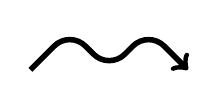
\begin{tikzpicture}[x=1mm,y=1mm]
  \draw[line width=2pt, rounded corners=8pt, ->]
  (0,0) -- (5,5) -- (10,0) -- (15,5) -- (20,0);
\end{tikzpicture}
が描かれる。
矢印は \verb'->'、\verb'<-'、\verb'<->'、\verb'->>' などが指定できる。
また、矢印の形には Ti\textit{k}Z 標準(
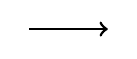
\begin{tikzpicture}[line width=1pt]
  \draw[->] (0,1) -- (1,1);
\end{tikzpicture}
)、\LaTeX{}標準(
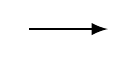
\begin{tikzpicture}[line width=1pt]
  \draw[-latex] (0,0.5) -- (1,0.5);
\end{tikzpicture}
)、ステルス戦闘機型(
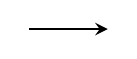
\begin{tikzpicture}[line width=1pt]
  \draw[-stealth] (0,0) -- (1,0);
\end{tikzpicture}
)などが用意されている。
\vspc{+0.50zw}\begin{mdframed}[roundcorner=0.50zw,leftmargin=3.00zw,rightmargin=3.00zw,skipabove=0.40zw,skipbelow=0.40zw,innertopmargin=4.00pt,innerbottommargin=4.00pt,innerleftmargin=5.00pt,innerrightmargin=5.00pt,linecolor=gray!020,linewidth=0.50pt,backgroundcolor=gray!20]
\begin{verbatim}
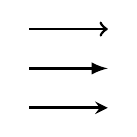
\begin{tikzpicture}[line width=1pt]
  \draw[->] (0,1) -- (1,1);
  \draw[-latex] (0,0.5) -- (1,0.5);
  \draw[-stealth] (0,0) -- (1,0);
\end{tikzpicture}
\end{verbatim}
\end{mdframed}\vspc{-0.70zw}
Ti\textit{k}Z 標準は、数式で $f:A \to B$ と書く際の \verb'\to'(\verb'\rightarrow')と(大きさは異なるが)同じ形である。\\

\verb'\draw' でグリッドや円、長方形、楕円も描くことができる。
勿論、日本語や数式も書くことができる。
\verb'\fill' にすると、指定した色で塗りつぶす(この例では 20\% の灰色)。
\vspc{+0.50zw}\begin{mdframed}[roundcorner=0.50zw,leftmargin=3.00zw,rightmargin=3.00zw,skipabove=0.40zw,skipbelow=0.40zw,innertopmargin=4.00pt,innerbottommargin=4.00pt,innerleftmargin=5.00pt,innerrightmargin=5.00pt,linecolor=gray!020,linewidth=0.50pt,backgroundcolor=gray!20]
\begin{verbatim}
\begin{tikzpicture}
  \draw[step=1,gray] (-0.2,-0.2) grid (2.2,2.2);
  \draw (0.5,0.5) circle (0.5) node {$\pi r^{2}$};
  \draw[line width=1pt] (1,0) rectangle (2,0.5);
  \fill[black!20] (1,1.5) ellipse (1 and 0.5);
  \draw (1,1.5) node {\hbox{\tate 楕円}};
\end{tikzpicture}
\end{verbatim}
\end{mdframed}\vspc{-0.70zw}
出力は次のようになる\\
\vspc{-2.50zw}\begin{center}
  \begin{tikzpicture}
    \draw[step=1,gray] (-0.2,-0.2) grid (2.2,2.2);
    \draw (0.5,0.5) circle (0.5) node {$\pi r^{2}$};
    \draw[line width=1pt] (1,0) rectangle (2,0.5);
    \fill[black!20] (1,1.5) ellipse (1 and 0.5);
    \draw (1,1.5) node {\hbox{\tate 楕円}};
  \end{tikzpicture}
\end{center}\vspc{-1.50zw}
より複雑な図形は、制御点を2つ与えたベジェ(B\'{e}zier)曲線で描くことができる。\enlargethispage{+0.90zw}
第 2 の制御点が第 1 のものと同じ場合は省略することができる。
\vspc{+0.50zw}\begin{mdframed}[roundcorner=0.50zw,leftmargin=3.00zw,rightmargin=3.00zw,skipabove=0.40zw,skipbelow=0.40zw,innertopmargin=4.00pt,innerbottommargin=4.00pt,innerleftmargin=5.00pt,innerrightmargin=5.00pt,linecolor=gray!020,linewidth=0.50pt,backgroundcolor=gray!20]
\begin{verbatim}
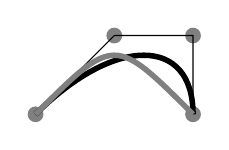
\begin{tikzpicture}[x=1mm,y=1mm]
  \fill[gray] ( 0, 0) circle (1)
              (10,10) circle (1)
              (20,10) circle (1)
              (20, 0) circle (1);
  \draw (0,0) -- (10,10) -- (20,10) -- (20,0);
  \draw[line width=2pt] (0,0) .. controls (10,10) and (20,10) .. (20,0);
  \draw[line width=2pt,gray] (0,0) .. controls (10,10) .. (20,0);
\end{tikzpicture}
\end{verbatim}
\end{mdframed}\vspc{-0.70zw}
出力は次のようになる。
\vspc{-1.50zw}\begin{center}
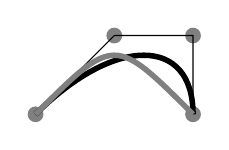
\begin{tikzpicture}[x=1mm,y=1mm]
  \fill[gray] ( 0, 0) circle (1)
              (10,10) circle (1)
              (20,10) circle (1)
              (20, 0) circle (1);
  \draw (0,0) -- (10,10) -- (20,10) -- (20,0);
  \draw[line width=2pt] (0,0) .. controls (10,10) and (20,10) .. (20,0);
  \draw[line width=2pt,gray] (0,0) .. controls (10,10) .. (20,0);
\end{tikzpicture}
\end{center}\vspc{-1.00zw}
折れ線と曲線は次のように混在させることができる。
\vspc{+0.00zw}\begin{mdframed}[roundcorner=0.50zw,leftmargin=3.00zw,rightmargin=3.00zw,skipabove=0.40zw,skipbelow=0.40zw,innertopmargin=4.00pt,innerbottommargin=4.00pt,innerleftmargin=5.00pt,innerrightmargin=5.00pt,linecolor=gray!020,linewidth=0.50pt,backgroundcolor=gray!20]
\begin{verbatim}

\begin{tikzpicture}[x=1mm,y=1mm,line width=2pt]
  \draw ( 2,2) circle (2);
  \draw ( 2,4) -- (6,4) -- ( 6,0) .. controls (6,3) and (7,4) ..
        (12,4) -- (9,0) -- (12,0);
\end{tikzpicture}
\end{verbatim}
\end{mdframed}\vspc{-0.70zw}
出力は次のようになる。
\vspc{-1.00zw}\begin{center}
  
\begin{tikzpicture}[x=1mm,y=1mm,line width=2pt]
    \draw (2,2) circle (2);
    \draw (2,4) -- (6,4) -- (6,0) .. controls (6,3) and (7,4) .. (12,4) -- (9,0) -- (12,0);
  \end{tikzpicture}
\end{center}\vspc{-1.00zw}
繰り返しも \verb'\foreach' という強力な命令で簡単に実現できる。
\verb'...' は書くのを省略したのではなく、本当にこのように記述すれば Ti\textit{k}Z が補ってくれる。
\vspc{+0.50zw}\begin{mdframed}[roundcorner=0.50zw,leftmargin=3.00zw,rightmargin=3.00zw,skipabove=0.40zw,skipbelow=0.40zw,innertopmargin=4.00pt,innerbottommargin=4.00pt,innerleftmargin=5.00pt,innerrightmargin=5.00pt,linecolor=gray!020,linewidth=0.50pt,backgroundcolor=gray!20]
\begin{verbatim}
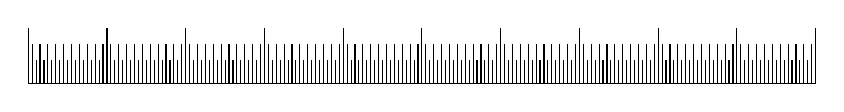
\begin{tikzpicture}[x=1mm,y=1mm]
  \draw (0,0) -- (100,0);
  \foreach \x in {0.0,...,100}    \draw (\x,0) -- (\x,3);
  \foreach \x in {0.5,...,100}    \draw (\x,0) -- (\x,5);
  \foreach \x in {0.0,10,...,100} \draw (\x,0) -- (\x,7);
\end{tikzpicture}
\end{verbatim}
\end{mdframed}\vspc{-0.70zw}
出力は次のようになる。
\vspc{-0.50zw}\begin{center}
  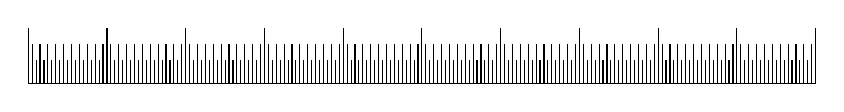
\begin{tikzpicture}[x=1mm,y=1mm]
  \draw (0,0) -- (100,0);
  \foreach \x in {0.0,...,100}    \draw (\x,0) -- (\x,3);
  \foreach \x in {0.5,...,100}    \draw (\x,0) -- (\x,5);
  \foreach \x in {0.0,10,...,100} \draw (\x,0) -- (\x,7);
\end{tikzpicture}
\end{center}\vspc{-0.50zw}
応用として、センター試験でよく使われる楕円の番号を作成してみる。
\vspc{+0.50zw}\begin{mdframed}[roundcorner=0.50zw,leftmargin=3.00zw,rightmargin=3.00zw,skipabove=0.40zw,skipbelow=0.40zw,innertopmargin=4.00pt,innerbottommargin=4.00pt,innerleftmargin=5.00pt,innerrightmargin=5.00pt,linecolor=gray!020,linewidth=0.50pt,backgroundcolor=gray!20]
\begin{verbatim}
\newcommand{\egg}[1]{\raisebox{-3pt}{%
    \begin{tikzpicture}[x=1pt,y=1pt,line width=1pt]
      \draw (0,0) ellipse (4.5 and 6);
      \draw (0,0) node {\fontfamily{phv}\fontsize{9pt}{0}\selectfont #1\/};
    \end{tikzpicture}}}
\newcommand{\eggg}[1]{\raisebox{-3pt}{%
    \begin{tikzpicture}[x=1pt,y=1pt,line width=1pt]
      \draw[fill=black!30] (0,0) ellipse (4.5 and 6);
      \draw (0,0) node {\fontfamily{phv}\fontsize{9pt}{0}\selectfont #1\/};
    \end{tikzpicture}}}
\end{verbatim}
\end{mdframed}\vspc{-0.70zw}
\newcommand{\egg}[1]{\raisebox{-3pt}{%
    \begin{tikzpicture}[x=1pt,y=1pt,line width=1pt]
      \draw (0,0) ellipse (4.5 and 6);
      \draw (0,0) node {\fontfamily{phv}\fontsize{9pt}{0}\selectfont #1\/};
    \end{tikzpicture}}}
\newcommand{\eggg}[1]{\raisebox{-3pt}{%
    \begin{tikzpicture}[x=1pt,y=1pt,line width=1pt]
      \draw[fill=black!30] (0,0) ellipse (4.5 and 6);
      \draw (0,0) node {\fontfamily{phv}\fontsize{9pt}{0}\selectfont #1\/};
    \end{tikzpicture}}}
これで \verb'\egg{0} \egg{1} \egg{2} \eggg{0} \eggg{1} \eggg{2}' とすれば \egg{0} \egg{1} \egg{2} \eggg{0} \eggg{1} \eggg{2} と出力される。\\
\renewcommand{\keytop}[2][12]{%
  \begin{tikzpicture}[x=0.1em,y=0.1em]
    \useasboundingbox (0,0) rectangle (#1,9);
    \shadedraw[top color=black!20,rounded corners=0.2em] (0,-3) rectangle (#1,9);
    \draw[anchor=base] (#1/2,0) node {\sffamily #2};
  \end{tikzpicture}}
次は \keytop{A} のようなキーボード記号である。
\vspc{+0.50zw}\begin{mdframed}[roundcorner=0.50zw,leftmargin=3.00zw,rightmargin=3.00zw,skipabove=0.40zw,skipbelow=0.40zw,innertopmargin=4.00pt,innerbottommargin=4.00pt,innerleftmargin=5.00pt,innerrightmargin=5.00pt,linecolor=gray!020,linewidth=0.50pt,backgroundcolor=gray!20]
\begin{verbatim}
\renewcommand{\keytop}[2][12]{%
  \begin{tikzpicture}[x=0.1em,y=0.1em]
    \useasboundingbox (0,0) rectangle (#1,9);
    \shadedraw[top color=black!20,rounded corners=0.2em] (0,-3)
    rectangle (#1,9);
    \draw[anchor=base] (#1/2,0) node {\sffamily #2};
\end{verbatim}
\end{mdframed}\vspc{-0.70zw}
\verb'\keytop{A}' と書けば \keytop{A} と出力される。
\keytop[30]{Enter} のように幅の広いものは \verb'\ketop[30]{Enter}' のように幅を 0.1em 単位で指定する。\enlargethispage{+1.00zw}
%%
%% 節:グラフの描画(1)
%%--------------------------------------------------------------------------------------------------------------------%%
\section{グラフの描画(1)}
Ti\textit{k}Z では \textrm{sin}、\textrm{cos}、\textrm{exp}、\textrm{sqrt} などの関数が利用できる。
但し、TeX{}で実装しているので、遅く、精度の低い固定小数点数である。
次のような簡単なことは可能である。
\vspc{+0.50zw}\begin{mdframed}[roundcorner=0.50zw,leftmargin=3.00zw,rightmargin=3.00zw,skipabove=0.40zw,skipbelow=0.40zw,innertopmargin=4.00pt,innerbottommargin=4.00pt,innerleftmargin=5.00pt,innerrightmargin=5.00pt,linecolor=gray!020,linewidth=0.50pt,backgroundcolor=gray!20]
\begin{verbatim}
\begin{tikzpicture}[domain=0:4,samples=200,>=stealth]
  \draw[->] (-0.5,0) -- (4.2,0) node[right] {$x$};
  \draw[->] (0,-0.5) -- (0,2.2) node[above] {$y$};
  \draw plot (\x, {sqrt(\x)}) node[below] {$y=\sqrt{x}$};
  \draw (0,0) node[below left] {O};
\end{tikzpicture}
\end{verbatim}
\end{mdframed}\vspc{-0.70zw}
出力は次のようになる。
\vspc{-0.50zw}\begin{center}
  \begin{tikzpicture}[domain=0:4,samples=200,>=stealth]
    \draw[->] (-0.5,0) -- (4.2,0) node[right] {$x$};
    \draw[->] (0,-0.5) -- (0,2.2) node[above] {$y$};
    \draw plot (\x, {sqrt(\x)}) node[below] {$y=\sqrt{x}$};
    \draw (0,0) node[below left] {O};
  \end{tikzpicture}
\end{center}\vspc{-0.50zw}
数値の表を与えてグラフをプロットすることもできる。
例えば、毎年の日本の合計特殊出生率が、
\vspc{-0.50zw}\begin{quote}
  1970 2.13 \\
  1971 2.16 \\
  1972 2.14 \\
  $\ldots$  \\
  2015 1.46
\end{quote}\vspc{-0.50zw}
のようなテキストファイル TFR.tbl で与えられているとする。
これを、
\begin{center}
  \begin{tikzpicture}[x=2mm,y=40mm]
    \draw (1968,1.2) -- (1968,2.2);
    \foreach \x in {1.2,1.4,1.6,1.8,2.0,2.2}
    \draw (1968,\x) -- (1967,\x) node[left] {\x};
    \draw (1970,1.1) -- (2015,1.1);
    \foreach \x in {1970,1980,...,2000,2010,2015}
    \draw (\x,1.1) -- (\x,1.05) node[below] {\x};
    \draw[mark=*] plot file {./Fig/TFR.tbl} node[above] {1.46};
  \end{tikzpicture}
\end{center}\vspc{-0.50zw}
のように描くには次のようにする。\enlargethispage{+0.50zw}
\vspc{+0.50zw}\begin{mdframed}[roundcorner=0.50zw,leftmargin=3.00zw,rightmargin=3.00zw,skipabove=0.40zw,skipbelow=0.40zw,innertopmargin=4.00pt,innerbottommargin=4.00pt,innerleftmargin=5.00pt,innerrightmargin=5.00pt,linecolor=gray!020,linewidth=0.50pt,backgroundcolor=gray!20]
\begin{verbatim}
\begin{tikzpicture}[x=2mm,y=40mm]
  \draw (1968,1.2) -- (1968,2.2);
  \foreach \x in {1.2,1.4,1.6,1.8,2.0,2.2}
  \draw (1968,\x) -- (1967,\x) node[left] {\x};
  \draw (1970,1.1) -- (2015,1.1);
  \foreach \x in {1970,1980,...,2000,2010,2015}
  \draw (\x,1.1) -- (\x,1.05) node[below] {\x};
  \draw[mark=*] plot file {TFR.tbl} node[above] {1.46};
\end{tikzpicture}
\end{verbatim}
\end{mdframed}\vspc{-0.50zw}
あるいは、もっと単純に
\begin{tikzpicture}[x=1pt]
  \fill (1970,2.13) circle (2pt) node[left] {2.13};
  \draw plot file {./Fig/TFR.tbl};
  \fill (2015,1.46) circle (2pt) node[right] {1.46};
\end{tikzpicture}
のようなスパークライン(sparkline)で描くには次のようにする。
\vspc{-1.00zw}\begin{mdframed}[roundcorner=0.50zw,leftmargin=3.00zw,rightmargin=3.00zw,skipabove=0.40zw,skipbelow=0.40zw,innertopmargin=4.00pt,innerbottommargin=4.00pt,innerleftmargin=5.00pt,innerrightmargin=5.00pt,linecolor=gray!020,linewidth=0.50pt,backgroundcolor=gray!20]
\begin{verbatim}
\begin{tikzpicture}[x=1pt]
  \fill (1970,2.13) circle (2pt) node[left] {2.13};
  \draw plot file {TFR.tbl};
  \fill (2015,1.46) circle (2pt) node[right] {1.46};
\end{tikzpicture}
\end{verbatim}
\end{mdframed}\vspc{-0.70zw}
但し、Ti\textit{k}Z は\TeX{}の固定小数点数で計算するので、あまり大きな値を扱うと ``ERROR:~Dimension too large.'' となることがある。
その場合は、適当に数値を切り詰める。\\

次の棒グラフの例では、年から 2000 を引いた値を$x$座標としている。
\vspc{+0.50zw}\begin{mdframed}[roundcorner=0.50zw,leftmargin=3.00zw,rightmargin=3.00zw,skipabove=0.40zw,skipbelow=0.40zw,innertopmargin=4.00pt,innerbottommargin=4.00pt,innerleftmargin=5.00pt,innerrightmargin=5.00pt,linecolor=gray!020,linewidth=0.50pt,backgroundcolor=gray!20]
\begin{verbatim}
\begin{tikzpicture}[ybar,x=5mm,y=0.005mm]
  \draw[fill=lightgray] plot coordinates
  {( 4,12415) ( 5,12317) ( 6,12214) ( 7,12043) ( 8,11813) ( 9,11695)
   (10,11585) (11,11528) (12,11366) (13,10792) (14,11123) (15,10945)};
  \draw (4,0) node[below] {2004};
  \draw (15,0) node[below] {2015};
  \draw (4,12315)|-(16,13000) node[right] {12415億円};
  \draw (15,10945)|-(16,12000) node[right] {10945億円};
  \draw (9.5,13000) node[above] {\large 国立大学運営費交付金};
\end{tikzpicture}
\end{verbatim}
\end{mdframed}\vspc{-0.70zw}
この例では、引出線を引くために \verb'--' ではなく \verb'|-' を使っている。
$(x_{1},y_{1})$ \verb'|-' $(x_{2},y_{2})$ は $(x_{1},y_{1})$ \verb'--' $(x_{1},y_{2})$ \verb'--' $(x_{2},y_{2})$ と同じことで、先に水平方向に、次に水平方向に線を引く。
水平と垂直の順序を入れ替えた \verb'-|' も用意されている。
\vspc{+0.50zw}\begin{center}
  \begin{tikzpicture}[ybar,x=5mm,y=0.005mm]
    \draw[fill=lightgray] plot coordinates
    {( 4,12415) ( 5,12317) ( 6,12214) ( 7,12043) ( 8,11813) ( 9,11695)
     (10,11585) (11,11528) (12,11366) (13,10792) (14,11123) (15,10945)};
    \draw (4,0) node[below] {2004};
    \draw (15,0) node[below] {2015};
    \draw (4,12315)|-(16,13000) node[right] {12415億円};
    \draw (15,10945)|-(16,12000) node[right] {10945億円};
    \draw (9.5, 13000) node[above] {\large 国立大学運営費交付金};
  \end{tikzpicture}
\end{center}\vspc{-0.70zw}
%%
%% 節:グラフの描画(2)
%%--------------------------------------------------------------------------------------------------------------------%%
\section{グラフの描画(2)}
グラフと言えば、グラフ理論のグラフも簡単に描くことができる。
ノード(点)に名前を付け、両端のノードを指定して辺を描けばよい。
次のグラフは、有名な \ruby{K\"{o}nigsberg}{ケーニヒスベルク} の橋の問題のグラフである。
\vspc{+0.50zw}\begin{mdframed}[roundcorner=0.50zw,leftmargin=3.00zw,rightmargin=3.00zw,skipabove=0.40zw,skipbelow=0.40zw,innertopmargin=4.00pt,innerbottommargin=4.00pt,innerleftmargin=5.00pt,innerrightmargin=5.00pt,linecolor=gray!020,linewidth=0.50pt,backgroundcolor=gray!20]
\begin{verbatim}
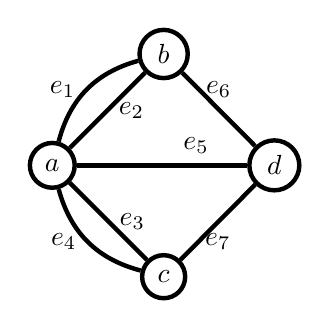
\begin{tikzpicture}[line width=1.6pt,node distance=2cm]
  \node(a) [draw,circle]{$a$};
  \node[above right of=a](b)                [draw,circle]{$b$};
  \node[below right of=a](c)                [draw,circle]{$c$};
  \node[right of=a,node distance=2.82cm](d) [draw,circle]{$d$};
  \draw (a) to[bend left]  node[midway,left]  {$e_{1}$} (b);
  \draw (a) --             node[midway,right] {$e_{2}$} (b);
  \draw (a) --             node[midway,right] {$e_{3}$} (c);
  \draw (a) to[bend right] node[midway,left]  {$e_{4}$} (c);
  \draw (a) --             node[pos=.7,above] {$e_{5}$} (d);
  \draw (b) --             node[midway,above] {$e_{6}$} (d);
  \draw (c) --             node[midway,below] {$e_{7}$} (d);
\end{tikzpicture}
\end{verbatim}
\end{mdframed}\vspc{-0.70zw}
\begin{center}
  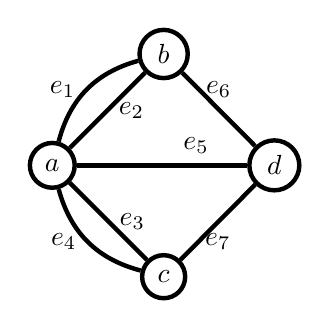
\begin{tikzpicture}[line width=1.6pt,node distance=2cm]
  \node(a) [draw,circle]{$a$};
  \node[above right of=a](b)                [draw,circle]{$b$};
  \node[below right of=a](c)                [draw,circle]{$c$};
  \node[right of=a,node distance=2.82cm](d) [draw,circle]{$d$};
  \draw (a) to[bend left]  node[midway,left]  {$e_{1}$} (b);
  \draw (a) --             node[midway,right] {$e_{2}$} (b);
  \draw (a) --             node[midway,right] {$e_{3}$} (c);
  \draw (a) to[bend right] node[midway,left]  {$e_{4}$} (c);
  \draw (a) --             node[pos=.7,above] {$e_{5}$} (d);
  \draw (b) --             node[midway,above] {$e_{6}$} (d);
  \draw (c) --             node[midway,below] {$e_{7}$} (d);
  \end{tikzpicture}
\end{center}
この例では、ノード$a$を基準とした相対的な位置で$b$、$c$、$d$を指定している。
辺は両端点で指定し、辺の途中にラベルを付けている。
bend left や bend right で湾曲した辺を描くには \verb'--'ではなく to を用いる(この例では \verb'--' を全て to に置き換えても構わない)。
%%
%% 節:gnuplot との連携
%%--------------------------------------------------------------------------------------------------------------------%%
\section{gnuplot との連携}
\ruby{gnuplot}{ニュープロット}\footnote{GNU プロジェクトを思わせる名前なのでグニュ―プロットと呼ばれることもあるが、GNU プロジェクトとは無関係である。} は昔から使われている強力なプロットツールである。
これと連携させて Ti\textit{k}Z のプロットを描くことができる。
例えば、標準正規分布のグラフを描いてみる。
次のように \verb'function{...}' という命令を使えば、関数の中身 \verb'exp(-x**2/2)/sqrt(2*pi)' が gnuplot に渡され、関数値の表に変換される。
この際、platex に \verb'-shell-escape' オプションを付けて起動しなければならない。
gnuplot で渡される命令と、返される表のファイル名は\LaTeX{}文書のファイル名と \verb'-id=' で与えられた名前から生成される。
一旦これらが生成されれば、関数を変えない限り gnuplot を呼び出すことはないので \verb'-shell-escape' オプションも不要である。\\
\vspc{-1.00zw}\begin{mdframed}[roundcorner=0.50zw,leftmargin=3.00zw,rightmargin=3.00zw,skipabove=0.40zw,skipbelow=0.40zw,innertopmargin=4.00pt,innerbottommargin=4.00pt,innerleftmargin=5.00pt,innerrightmargin=5.00pt,linecolor=gray!020,linewidth=0.50pt,backgroundcolor=gray!20]
\begin{verbatim}
\begin{tikzpicture}[domain=-3:3,samples=50,>=latex,y=8cm]
  \draw[->] (-3.2,0) -- (3.2,0) node[right] {$x$};
  \draw plot[id=dnorm,smooth] function{exp(-x**2/2)/sqrt(2*pi)};
  \draw (2,0.35) node {$y=\frac{1}{\sqrt{2\pi}}e^{-x^{2}\!\/2}$};
  \foreach \x in {-3,...,3}
  \draw (\x,0) -- (\x,-0.02) node[below=-2pt] {\footnotesize $\x$};
\end{tikzpicture}
\end{verbatim}
\end{mdframed}\vspc{-0.70zw}
\begin{center}
  \begin{tikzpicture}[domain=-3:3,samples=50,>=latex,y=8cm]
    \draw[->] (-3.2,0) -- (3.2,0) node[right] {$x$};
    \draw plot[id=dnorm,smooth] function{exp(-x**2/2)/sqrt(2*pi)};
    \draw (2,0.35) node {$y=\frac{1}{\sqrt{2\pi}}e^{-x^{2}\!\/2}$};
    \foreach \x in {-3,...,3}
    \draw (\x,0) -- (\x,-0.02) node[below=-2pt] {\footnotesize $\x$};
  \end{tikzpicture}
\end{center}
尚、これぐらいの関数であれば、Ti\textit{k}Z だけで、
\vspc{+0.50zw}\begin{mdframed}[roundcorner=0.50zw,leftmargin=3.00zw,rightmargin=3.00zw,skipabove=0.40zw,skipbelow=0.40zw,innertopmargin=4.00pt,innerbottommargin=4.00pt,innerleftmargin=5.00pt,innerrightmargin=5.00pt,linecolor=gray!020,linewidth=0.50pt,backgroundcolor=gray!20]
\begin{verbatim}
\draw plot[smooth] (\x, {exp(-0.5 * \x \x) / sqrt(2 * pi)});
\end{verbatim}
\end{mdframed}\vspc{-0.70zw}
のようにして描くこともできる。\\

gnuplot から返される表は、\# で始まるコメント行を除けば、次のような形式である。
\vspc{+0.50zw}\begin{mdframed}[roundcorner=0.50zw,leftmargin=3.00zw,rightmargin=3.00zw,skipabove=0.40zw,skipbelow=0.40zw,innertopmargin=4.00pt,innerbottommargin=4.00pt,innerleftmargin=5.00pt,innerrightmargin=5.00pt,linecolor=gray!020,linewidth=0.50pt,backgroundcolor=gray!20]
\begin{verbatim}
  -3.00000 0.00443 i
  -2.87755 0.00635 i
  -2.75510 0.00897 i
  ...
\end{verbatim}
\end{mdframed}\vspc{-0.70zw}
最後の文字 i は範囲内、o は範囲外、u は未定義を表す。\enlargethispage{+0.60zw}
gnuplot に関わらず、このような表を用意しておけば、
\vspc{+0.50zw}\begin{mdframed}[roundcorner=0.50zw,leftmargin=3.00zw,rightmargin=3.00zw,skipabove=0.40zw,skipbelow=0.40zw,innertopmargin=4.00pt,innerbottommargin=4.00pt,innerleftmargin=5.00pt,innerrightmargin=5.00pt,linecolor=gray!020,linewidth=0.50pt,backgroundcolor=gray!20]
\begin{verbatim}
\draw plot[smooth] file {ファイル名};
\end{verbatim}
\end{mdframed}\vspc{-0.70zw}
のようにしてプロットすることができる。

別の方法として gnuplot で、
\vspc{+0.50zw}\begin{mdframed}[roundcorner=0.50zw,leftmargin=3.00zw,rightmargin=3.00zw,skipabove=0.40zw,skipbelow=0.40zw,innertopmargin=4.00pt,innerbottommargin=4.00pt,innerleftmargin=5.00pt,innerrightmargin=5.00pt,linecolor=gray!020,linewidth=0.50pt,backgroundcolor=gray!20]
\begin{verbatim}
set term tikz
\end{verbatim}
\end{mdframed}\vspc{-0.70zw}
とすれば、Ti\textit{k}Z 形式の出力が得られる。
例えば、
\vspc{+0.50zw}\begin{mdframed}[roundcorner=0.50zw,leftmargin=3.00zw,rightmargin=3.00zw,skipabove=0.40zw,skipbelow=0.40zw,innertopmargin=4.00pt,innerbottommargin=4.00pt,innerleftmargin=5.00pt,innerrightmargin=5.00pt,linecolor=gray!020,linewidth=0.50pt,backgroundcolor=gray!20]
\begin{verbatim}
set term tikz monochrome
set output "dnorm-gp.tex"
set xrange [-3:3]
plot exp(-x**2/2)/sqrt(2*pi) with lines
exit
\end{verbatim}
\end{mdframed}\vspc{-0.70zw}
とし、\LaTeX{}文書の中では、
\vspc{+0.50zw}\begin{mdframed}[roundcorner=0.50zw,leftmargin=3.00zw,rightmargin=3.00zw,skipabove=0.40zw,skipbelow=0.40zw,innertopmargin=4.00pt,innerbottommargin=4.00pt,innerleftmargin=5.00pt,innerrightmargin=5.00pt,linecolor=gray!020,linewidth=0.50pt,backgroundcolor=gray!20]
\begin{verbatim}
\documentclass[dvipdfmx]{jsarticle}
\usepackage{gnuplot-lua-tikz}
\begin{document}
\begin{tikzpicture}[gnuplot]
%% generated with GNUPLOT 5.2p8 (Lua 5.3; terminal rev. Nov 2018, script rev. 108)
%% 2020年09月17日 09時41分47秒
\path (0.000,0.000) rectangle (12.500,8.750);
\gpcolor{color=gp lt color border}
\gpsetlinetype{gp lt border}
\gpsetdashtype{gp dt solid}
\gpsetlinewidth{1.00}
\draw[gp path] (1.196,0.616)--(1.376,0.616);
\draw[gp path] (11.947,0.616)--(11.767,0.616);
\node[gp node right] at (1.012,0.616) {$0$};
\draw[gp path] (1.196,1.594)--(1.376,1.594);
\draw[gp path] (11.947,1.594)--(11.767,1.594);
\node[gp node right] at (1.012,1.594) {$0.05$};
\draw[gp path] (1.196,2.572)--(1.376,2.572);
\draw[gp path] (11.947,2.572)--(11.767,2.572);
\node[gp node right] at (1.012,2.572) {$0.1$};
\draw[gp path] (1.196,3.550)--(1.376,3.550);
\draw[gp path] (11.947,3.550)--(11.767,3.550);
\node[gp node right] at (1.012,3.550) {$0.15$};
\draw[gp path] (1.196,4.529)--(1.376,4.529);
\draw[gp path] (11.947,4.529)--(11.767,4.529);
\node[gp node right] at (1.012,4.529) {$0.2$};
\draw[gp path] (1.196,5.507)--(1.376,5.507);
\draw[gp path] (11.947,5.507)--(11.767,5.507);
\node[gp node right] at (1.012,5.507) {$0.25$};
\draw[gp path] (1.196,6.485)--(1.376,6.485);
\draw[gp path] (11.947,6.485)--(11.767,6.485);
\node[gp node right] at (1.012,6.485) {$0.3$};
\draw[gp path] (1.196,7.463)--(1.376,7.463);
\draw[gp path] (11.947,7.463)--(11.767,7.463);
\node[gp node right] at (1.012,7.463) {$0.35$};
\draw[gp path] (1.196,8.441)--(1.376,8.441);
\draw[gp path] (11.947,8.441)--(11.767,8.441);
\node[gp node right] at (1.012,8.441) {$0.4$};
\draw[gp path] (1.196,0.616)--(1.196,0.796);
\draw[gp path] (1.196,8.441)--(1.196,8.261);
\node[gp node center] at (1.196,0.308) {$-3$};
\draw[gp path] (2.988,0.616)--(2.988,0.796);
\draw[gp path] (2.988,8.441)--(2.988,8.261);
\node[gp node center] at (2.988,0.308) {$-2$};
\draw[gp path] (4.780,0.616)--(4.780,0.796);
\draw[gp path] (4.780,8.441)--(4.780,8.261);
\node[gp node center] at (4.780,0.308) {$-1$};
\draw[gp path] (6.572,0.616)--(6.572,0.796);
\draw[gp path] (6.572,8.441)--(6.572,8.261);
\node[gp node center] at (6.572,0.308) {$0$};
\draw[gp path] (8.363,0.616)--(8.363,0.796);
\draw[gp path] (8.363,8.441)--(8.363,8.261);
\node[gp node center] at (8.363,0.308) {$1$};
\draw[gp path] (10.155,0.616)--(10.155,0.796);
\draw[gp path] (10.155,8.441)--(10.155,8.261);
\node[gp node center] at (10.155,0.308) {$2$};
\draw[gp path] (11.947,0.616)--(11.947,0.796);
\draw[gp path] (11.947,8.441)--(11.947,8.261);
\node[gp node center] at (11.947,0.308) {$3$};
\draw[gp path] (1.196,8.441)--(1.196,0.616)--(11.947,0.616)--(11.947,8.441)--cycle;
\node[gp node right] at (10.479,8.107) {exp(-x**2/2)/sqrt(2*pi)};
\draw[gp path] (10.663,8.107)--(11.579,8.107);
\draw[gp path] (1.196,0.703)--(1.305,0.720)--(1.413,0.740)--(1.522,0.763)--(1.630,0.790)%
  --(1.739,0.822)--(1.848,0.858)--(1.956,0.899)--(2.065,0.946)--(2.173,1.000)--(2.282,1.061)%
  --(2.391,1.129)--(2.499,1.206)--(2.608,1.292)--(2.716,1.387)--(2.825,1.493)--(2.934,1.610)%
  --(3.042,1.738)--(3.151,1.878)--(3.259,2.030)--(3.368,2.194)--(3.477,2.372)--(3.585,2.562)%
  --(3.694,2.765)--(3.802,2.980)--(3.911,3.208)--(4.019,3.446)--(4.128,3.696)--(4.237,3.955)%
  --(4.345,4.223)--(4.454,4.498)--(4.562,4.779)--(4.671,5.063)--(4.780,5.350)--(4.888,5.636)%
  --(4.997,5.920)--(5.105,6.200)--(5.214,6.473)--(5.323,6.737)--(5.431,6.990)--(5.540,7.228)%
  --(5.648,7.451)--(5.757,7.654)--(5.866,7.838)--(5.974,7.999)--(6.083,8.135)--(6.191,8.247)%
  --(6.300,8.331)--(6.409,8.388)--(6.517,8.417)--(6.626,8.417)--(6.734,8.388)--(6.843,8.331)%
  --(6.952,8.247)--(7.060,8.135)--(7.169,7.999)--(7.277,7.838)--(7.386,7.654)--(7.495,7.451)%
  --(7.603,7.228)--(7.712,6.990)--(7.820,6.737)--(7.929,6.473)--(8.038,6.200)--(8.146,5.920)%
  --(8.255,5.636)--(8.363,5.350)--(8.472,5.063)--(8.581,4.779)--(8.689,4.498)--(8.798,4.223)%
  --(8.906,3.955)--(9.015,3.696)--(9.124,3.446)--(9.232,3.208)--(9.341,2.980)--(9.449,2.765)%
  --(9.558,2.562)--(9.666,2.372)--(9.775,2.194)--(9.884,2.030)--(9.992,1.878)--(10.101,1.738)%
  --(10.209,1.610)--(10.318,1.493)--(10.427,1.387)--(10.535,1.292)--(10.644,1.206)--(10.752,1.129)%
  --(10.861,1.061)--(10.970,1.000)--(11.078,0.946)--(11.187,0.899)--(11.295,0.858)--(11.404,0.822)%
  --(11.513,0.790)--(11.621,0.763)--(11.730,0.740)--(11.838,0.720)--(11.947,0.703);
\draw[gp path] (1.196,8.441)--(1.196,0.616)--(11.947,0.616)--(11.947,8.441)--cycle;
%% coordinates of the plot area
\gpdefrectangularnode{gp plot 1}{\pgfpoint{1.196cm}{0.616cm}}{\pgfpoint{11.947cm}{8.441cm}}
\end{tikzpicture}
%% gnuplot variables

\end{document}
\end{verbatim}
\end{mdframed}\vspc{-0.70zw}
とすれば、下のような図が得られる。
実際には、更に手を加えて見栄えを良くする必要がある。
\begin{center}
  \begin{tikzpicture}[gnuplot]
%% generated with GNUPLOT 5.2p8 (Lua 5.3; terminal rev. Nov 2018, script rev. 108)
%% 2020年09月17日 09時41分47秒
\path (0.000,0.000) rectangle (12.500,8.750);
\gpcolor{color=gp lt color border}
\gpsetlinetype{gp lt border}
\gpsetdashtype{gp dt solid}
\gpsetlinewidth{1.00}
\draw[gp path] (1.196,0.616)--(1.376,0.616);
\draw[gp path] (11.947,0.616)--(11.767,0.616);
\node[gp node right] at (1.012,0.616) {$0$};
\draw[gp path] (1.196,1.594)--(1.376,1.594);
\draw[gp path] (11.947,1.594)--(11.767,1.594);
\node[gp node right] at (1.012,1.594) {$0.05$};
\draw[gp path] (1.196,2.572)--(1.376,2.572);
\draw[gp path] (11.947,2.572)--(11.767,2.572);
\node[gp node right] at (1.012,2.572) {$0.1$};
\draw[gp path] (1.196,3.550)--(1.376,3.550);
\draw[gp path] (11.947,3.550)--(11.767,3.550);
\node[gp node right] at (1.012,3.550) {$0.15$};
\draw[gp path] (1.196,4.529)--(1.376,4.529);
\draw[gp path] (11.947,4.529)--(11.767,4.529);
\node[gp node right] at (1.012,4.529) {$0.2$};
\draw[gp path] (1.196,5.507)--(1.376,5.507);
\draw[gp path] (11.947,5.507)--(11.767,5.507);
\node[gp node right] at (1.012,5.507) {$0.25$};
\draw[gp path] (1.196,6.485)--(1.376,6.485);
\draw[gp path] (11.947,6.485)--(11.767,6.485);
\node[gp node right] at (1.012,6.485) {$0.3$};
\draw[gp path] (1.196,7.463)--(1.376,7.463);
\draw[gp path] (11.947,7.463)--(11.767,7.463);
\node[gp node right] at (1.012,7.463) {$0.35$};
\draw[gp path] (1.196,8.441)--(1.376,8.441);
\draw[gp path] (11.947,8.441)--(11.767,8.441);
\node[gp node right] at (1.012,8.441) {$0.4$};
\draw[gp path] (1.196,0.616)--(1.196,0.796);
\draw[gp path] (1.196,8.441)--(1.196,8.261);
\node[gp node center] at (1.196,0.308) {$-3$};
\draw[gp path] (2.988,0.616)--(2.988,0.796);
\draw[gp path] (2.988,8.441)--(2.988,8.261);
\node[gp node center] at (2.988,0.308) {$-2$};
\draw[gp path] (4.780,0.616)--(4.780,0.796);
\draw[gp path] (4.780,8.441)--(4.780,8.261);
\node[gp node center] at (4.780,0.308) {$-1$};
\draw[gp path] (6.572,0.616)--(6.572,0.796);
\draw[gp path] (6.572,8.441)--(6.572,8.261);
\node[gp node center] at (6.572,0.308) {$0$};
\draw[gp path] (8.363,0.616)--(8.363,0.796);
\draw[gp path] (8.363,8.441)--(8.363,8.261);
\node[gp node center] at (8.363,0.308) {$1$};
\draw[gp path] (10.155,0.616)--(10.155,0.796);
\draw[gp path] (10.155,8.441)--(10.155,8.261);
\node[gp node center] at (10.155,0.308) {$2$};
\draw[gp path] (11.947,0.616)--(11.947,0.796);
\draw[gp path] (11.947,8.441)--(11.947,8.261);
\node[gp node center] at (11.947,0.308) {$3$};
\draw[gp path] (1.196,8.441)--(1.196,0.616)--(11.947,0.616)--(11.947,8.441)--cycle;
\node[gp node right] at (10.479,8.107) {exp(-x**2/2)/sqrt(2*pi)};
\draw[gp path] (10.663,8.107)--(11.579,8.107);
\draw[gp path] (1.196,0.703)--(1.305,0.720)--(1.413,0.740)--(1.522,0.763)--(1.630,0.790)%
  --(1.739,0.822)--(1.848,0.858)--(1.956,0.899)--(2.065,0.946)--(2.173,1.000)--(2.282,1.061)%
  --(2.391,1.129)--(2.499,1.206)--(2.608,1.292)--(2.716,1.387)--(2.825,1.493)--(2.934,1.610)%
  --(3.042,1.738)--(3.151,1.878)--(3.259,2.030)--(3.368,2.194)--(3.477,2.372)--(3.585,2.562)%
  --(3.694,2.765)--(3.802,2.980)--(3.911,3.208)--(4.019,3.446)--(4.128,3.696)--(4.237,3.955)%
  --(4.345,4.223)--(4.454,4.498)--(4.562,4.779)--(4.671,5.063)--(4.780,5.350)--(4.888,5.636)%
  --(4.997,5.920)--(5.105,6.200)--(5.214,6.473)--(5.323,6.737)--(5.431,6.990)--(5.540,7.228)%
  --(5.648,7.451)--(5.757,7.654)--(5.866,7.838)--(5.974,7.999)--(6.083,8.135)--(6.191,8.247)%
  --(6.300,8.331)--(6.409,8.388)--(6.517,8.417)--(6.626,8.417)--(6.734,8.388)--(6.843,8.331)%
  --(6.952,8.247)--(7.060,8.135)--(7.169,7.999)--(7.277,7.838)--(7.386,7.654)--(7.495,7.451)%
  --(7.603,7.228)--(7.712,6.990)--(7.820,6.737)--(7.929,6.473)--(8.038,6.200)--(8.146,5.920)%
  --(8.255,5.636)--(8.363,5.350)--(8.472,5.063)--(8.581,4.779)--(8.689,4.498)--(8.798,4.223)%
  --(8.906,3.955)--(9.015,3.696)--(9.124,3.446)--(9.232,3.208)--(9.341,2.980)--(9.449,2.765)%
  --(9.558,2.562)--(9.666,2.372)--(9.775,2.194)--(9.884,2.030)--(9.992,1.878)--(10.101,1.738)%
  --(10.209,1.610)--(10.318,1.493)--(10.427,1.387)--(10.535,1.292)--(10.644,1.206)--(10.752,1.129)%
  --(10.861,1.061)--(10.970,1.000)--(11.078,0.946)--(11.187,0.899)--(11.295,0.858)--(11.404,0.822)%
  --(11.513,0.790)--(11.621,0.763)--(11.730,0.740)--(11.838,0.720)--(11.947,0.703);
\draw[gp path] (1.196,8.441)--(1.196,0.616)--(11.947,0.616)--(11.947,8.441)--cycle;
%% coordinates of the plot area
\gpdefrectangularnode{gp plot 1}{\pgfpoint{1.196cm}{0.616cm}}{\pgfpoint{11.947cm}{8.441cm}}
\end{tikzpicture}
%% gnuplot variables

\end{center}
%%
%% 節:他の図との重ね書き
%%--------------------------------------------------------------------------------------------------------------------%%
\section{他の図との重ね書き節}
Ti\textit{k}Z は強力な描画能力を備えているが、コマンドだけで全てを描くのは難しい。
そこで、他のソフトで描いた図の上に\TeX{}の数式などを Ti\textit{k}Z で重ね書きする方法を考える。
例えば、Ghostscript の虎の絵に説明を加えてみる。
図は、\enlargethispage{+0.50zw}
\vspc{-1.00zw}\begin{mdframed}[roundcorner=0.50zw,leftmargin=3.00zw,rightmargin=3.00zw,skipabove=0.40zw,skipbelow=0.40zw,innertopmargin=4.00pt,innerbottommargin=4.00pt,innerleftmargin=5.00pt,innerrightmargin=5.00pt,linecolor=gray!020,linewidth=0.50pt,backgroundcolor=gray!20]
\begin{verbatim}
\includegraphics[width=3cm]{tiger.pdf}
\end{verbatim}
\end{mdframed}\vspc{-0.70zw}
のような命令で読み込むのであった。\\

この任意の位置に文字や図を重ね書きするために、一時的にグラフ用紙を重ね書きしてみる。
\vspc{+0.50zw}\begin{mdframed}[roundcorner=0.50zw,leftmargin=3.00zw,rightmargin=3.00zw,skipabove=0.40zw,skipbelow=0.40zw,innertopmargin=4.00pt,innerbottommargin=4.00pt,innerleftmargin=5.00pt,innerrightmargin=5.00pt,linecolor=gray!020,linewidth=0.50pt,backgroundcolor=gray!20]
\begin{verbatim}
\begin{tikzpicture}[inner sep=0pt]
  \node[anchor=south west] (image) at (0,0)
       {\includegraphics[width=3cm]{tiger.pdf}};
  \draw[step=0.1,lightgray] (0,0) grid (image.north east);
  \draw[step=1,gray] (0,0) grid (image.noth east);
\end{tikzpicture}
\end{verbatim}
\end{mdframed}\vspc{-0.70zw}
\begin{center}
  \begin{tikzpicture}[inner sep=0pt]
    \node[anchor=south west] (image) at (0,0)
         {
\includegraphics[width=3cm]{./Fig/Fig09_01.PNG}};
         \draw[step=0.1,lightgray] (0,0) grid (image.north east);
         \draw[step=1,gray] (0,0) grid (image.north east);
  \end{tikzpicture}
\end{center}
これを見ながら、座標 $(0.3,2.5)$ の場所を中心とする位置に文字を入れてみる。
tikzpicture 環境内に追加するのは次の 2 行である。
\vspc{+0.50zw}\begin{mdframed}[roundcorner=0.50zw,leftmargin=3.00zw,rightmargin=3.00zw,skipabove=0.40zw,skipbelow=0.40zw,innertopmargin=4.00pt,innerbottommargin=4.00pt,innerleftmargin=5.00pt,innerrightmargin=5.00pt,linecolor=gray!020,linewidth=0.50pt,backgroundcolor=gray!20]
\begin{verbatim}
\node[white] at (0.3,2.5) {\hbox{\tate {\LARGE 虎}さん}};
\node at (0.2,0.3) {がおー};
\end{verbatim}
\end{mdframed}\vspc{-0.70zw}
うまくいったらグラフ用紙(grid)を描く次の 2 行は消しておく。
\vspc{+0.50zw}\begin{mdframed}[roundcorner=0.50zw,leftmargin=3.00zw,rightmargin=3.00zw,skipabove=0.40zw,skipbelow=0.40zw,innertopmargin=4.00pt,innerbottommargin=4.00pt,innerleftmargin=5.00pt,innerrightmargin=5.00pt,linecolor=gray!020,linewidth=0.50pt,backgroundcolor=gray!20]
\begin{verbatim}
\draw[step=0.1,lightgray] (0,0) grid (image.north east);
\draw[step=1,gray] (0,0) grid (image.north east);
\end{verbatim}
\end{mdframed}\vspc{-0.70zw}
結果は下のようになる。
\begin{center}
  \begin{tikzpicture}[inner sep=0pt]
    \node[anchor=south west] (image) at (0,0)
         {
\includegraphics[width=3cm]{./Fig/Fig09_01.PNG}};
    \node[white] at (0.3,2.5) {\hbox{\tate {\LARGE 虎}さん}};
    \node at (0.2,0.3) {がおー};
  \end{tikzpicture}
\end{center}
